\documentclass[aspectratio=169]{ctexbeamer}
\usepackage{booktabs}
\usepackage{listings}
\usepackage{xcolor}
\usepackage{float}
\usetheme{Madrid}

\beamertemplatenavigationsymbolsempty
\definecolor{tuna}{rgb}{0.098,0.51,0.696}
\definecolor{thu}{rgb}{0.50,0.36,0.71}

\setbeamercolor{section in toc}{fg=black,bg=white}
\setbeamercolor{item}{fg=tuna,bg=white}
\setbeamercolor{alerted text}{fg=tuna!80!gray}
\setbeamercolor*{palette primary}{fg=tuna!60!black,bg=gray!30!white}
\setbeamercolor*{palette secondary}{fg=tuna!70!black,bg=gray!15!white}
\setbeamercolor*{palette tertiary}{bg=tuna!80!black,fg=gray!10!white}
\setbeamercolor*{palette quaternary}{fg=tuna,bg=gray!5!white}

\setbeamercolor*{sidebar}{fg=tuna,bg=gray!15!white}

\setbeamercolor*{palette sidebar primary}{fg=tuna!10!black}
\setbeamercolor*{palette sidebar secondary}{fg=white}
\setbeamercolor*{palette sidebar tertiary}{fg=tuna!50!black}
\setbeamercolor*{palette sidebar quaternary}{fg=gray!10!white}

%\setbeamercolor*{titlelike}{parent=palette primary}
\setbeamercolor{titlelike}{parent=palette primary,fg=tuna}
\setbeamercolor{frametitle}{bg=gray!10!white}
\setbeamercolor{frametitle right}{bg=gray!60!white}

\setbeamercolor*{separation line}{}
\setbeamercolor*{fine separation line}{}

\setbeamertemplate{sections/subsections in toc}[square]
\setbeamertemplate{items}[square]

% Add "\usepackage{xcolor}"
% define some basic colors
\definecolor{mauve}{rgb}{0.58,0,0.82}

\definecolor{codegreen}{rgb}{0,0.6,0}
\definecolor{codegray}{rgb}{0.5,0.5,0.5}
\definecolor{codepurple}{rgb}{0.58,0,0.82}
\definecolor{backcolour}{rgb}{1,1,1}


\setmonofont{inconsolata}

\lstset{
% listings sonderzeichen (for german weirdness)
literate={ö}{{\"o}}1
{ä}{{\"a}}1
{ü}{{\"u}}1,
basicstyle=\tiny\ttfamily,                    % very small code
breaklines=true,                              % break long lines
commentstyle=\itshape\color{green!50!black},  % comments are green
keywordstyle=[1]\color{blue!80!black},        % instructions are blue
keywordstyle=[2]\color{orange!80!black},      % sections/other directives are orange
keywordstyle=[3]\color{red!50!black},         % registers are red
stringstyle=\color{mauve},                    % strings are from the telekom
identifierstyle=\color{teal},                 % user declared addresses are teal
frame=l,                                      % black line on the left side of code
language=C++,                   % all code is RISC-V
tabsize=4,                                    % indent tabs with 4 spaces
showstringspaces=false                        % do not replace spaces with weird underlines
}

\lstdefinestyle{mystyle}
{
    backgroundcolor=\color{backcolour},
    commentstyle=\color{codegreen},
    keywordstyle=\color{magenta},
    numberstyle=\tiny\color{codegray},
    stringstyle=\color{codepurple},
    basicstyle=\ttfamily\footnotesize,
    breakatwhitespace=false,
    breaklines=true,
    captionpos=b,
    keepspaces=true,
    numbers=none,
    numbersep=5pt,
    showspaces=false,
    showstringspaces=false,
    showtabs=false,
    tabsize=2,
    frame=none
}

\lstset{style=mystyle,language=C++}

\AtBeginSection[]{
    \begin{frame}
        \vfill
        \centering
        \begin{beamercolorbox}[sep=8pt,center,shadow=true,rounded=true]{title}
            \usebeamerfont{title}\insertsectionhead\par%
        \end{beamercolorbox}
        \vfill
    \end{frame}
}


\title{Auto Vectorization Methods \& Implementations for Modern Architecture}
\subtitle{现代体系结构自动向量化的方法与实现}
\author{龙英池}
\institute{Interns @ ISCAS}

\begin{document}
\maketitle
\section{Introduction}
\subsection{Challenges}
\begin{frame}
    \frametitle{Challenges - 并行的多样性}

    并行是目前主要算力,但是 ISA 定义多样。我们难以找到一个合适的抽象来用统一的范式进行自动向量化。

    \begin{table}
        \centering
        \begin{tabular}{ccc}
            \toprule
            设备 / ISA         & 对应的并行实现                             & 备注           \\
            \midrule
            NVIDIA/AMD GPU   & SIMT                                & 结合 SIMD 和多线程 \\
            寒武纪              & SIMD 长度可变                           & repeat 操作    \\
            升腾               & 默认操作 tensor                         & 看起来可能是多维的    \\
            以 x86 为代表的传统 CPU & 定长,通常可以同时操作标量                       & 需要对齐、尾循环处理等  \\
            RISC-V           & scatter \& gather, \& 长度可变, \& mask & V 扩展         \\
            ARM-SVE          & 类似 RVV                              & 没有 RVV 灵活    \\
            \bottomrule
        \end{tabular}
    \end{table}

    编译器难以使用统一的范式进行自动向量化。

\end{frame}

\subsection{Prior Art}

\begin{frame}
    \frametitle{Prior Art - MLIR \& LLVM}

    \begin{enumerate}
        \item MLIR - 目前没有自动向量化 \\
              Vector Dialect,面向各种 DSL 提供 n-D vector type,并可以在 lowering 到 LLVM IR 的过程中对 n-D vector 进行 re-layout,例如组成float4,
        \item LLVM - 有向量化,但主要面向传统 CPU \\
              从引入 Vector Predication 开始,主要被作为 CodeGen 的最后一关对接 MLIR,LLVM 本身的自动向量化有较大历史包袱。
    \end{enumerate}
\end{frame}

\subsection{Goal}

\begin{frame}
    \frametitle{Goal - Auto-Vectorization Service}

    \begin{enumerate}
        \item Extensible: 足够方便扩展
        \item Composible: 可以组合各种情况
        \item Simple: IR 层面尽量显然,避免多余静态分析
    \end{enumerate}
\end{frame}

\section{Virtual Vector - Vector Dialect}

\begin{frame}[fragile]
    \frametitle{Virtual Vector}

    MLIR Vector Dialect 提供了一个 nD vector 的抽象。这种抽象对于现代 HPC 来说是必要的。

    一个简单的例子:

    \begin{lstlisting}
kernel(float A).     load A[0-3]; add[0-3]
kernel (float4 A).     load A[0-15]; add[0-3] ; add[4-7]; add[]; add[]

vector A[100xfloat] => A[25* 4xfloat]
    \end{lstlisting}

\end{frame}

\begin{frame}
    \frametitle{Position}

    \begin{figure}
        \centering
        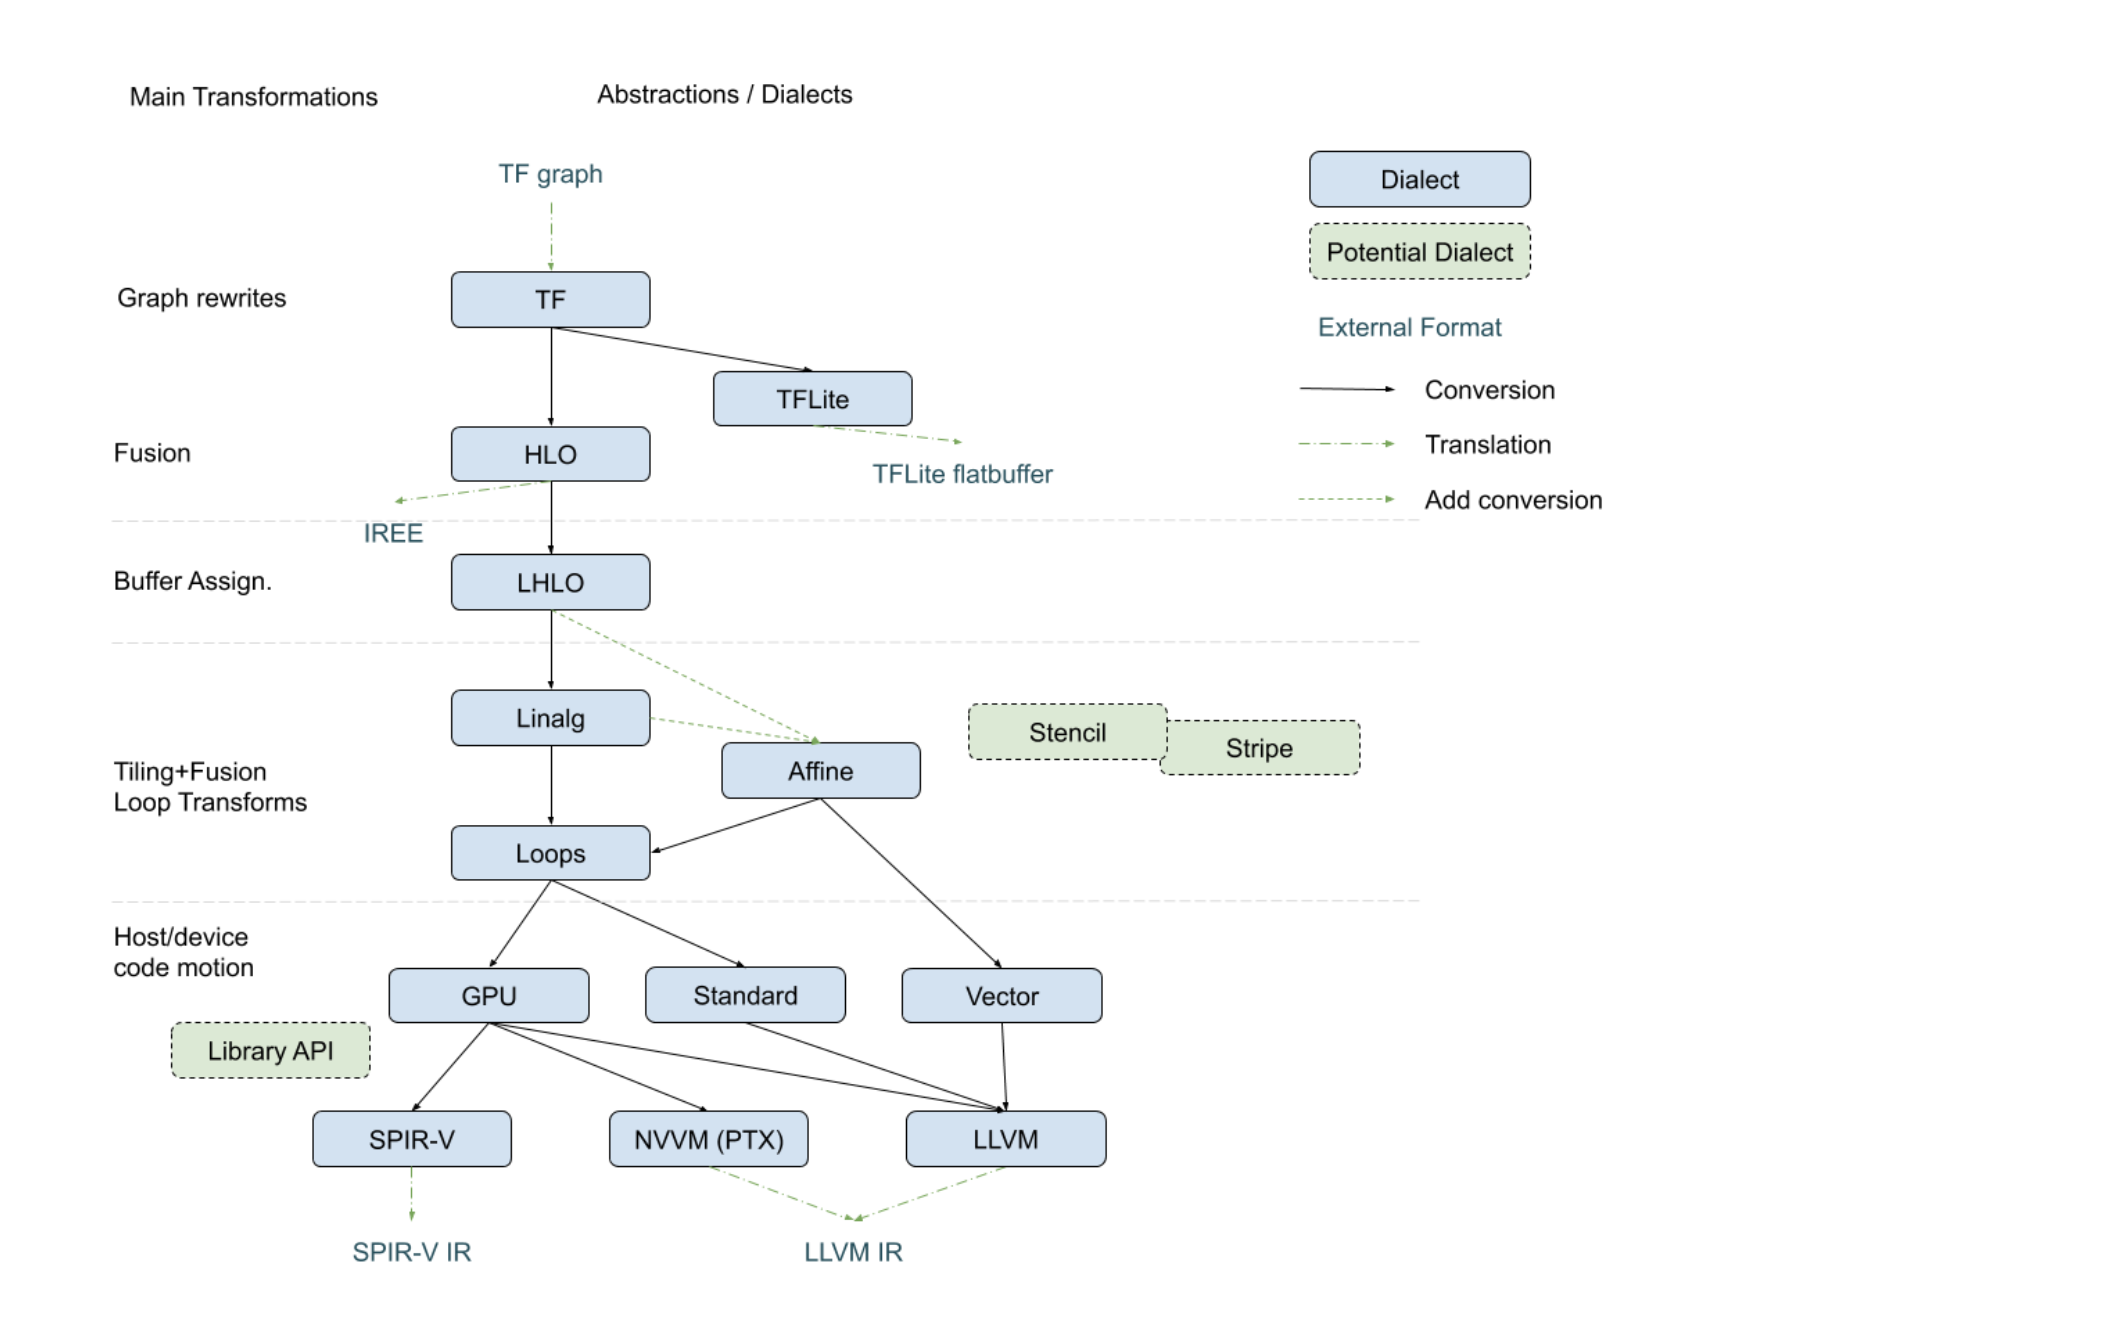
\includegraphics[width=0.56\linewidth]{images/position.png}
        \caption{Positioning in the Codegen Infrastructure}
    \end{figure}

\end{frame}

\begin{frame}
    \frametitle{Virtual Vector Lowering Path}
    \noindent
    \begin{minipage}[t]{0.50\linewidth}
        \begin{figure}
            \centering
            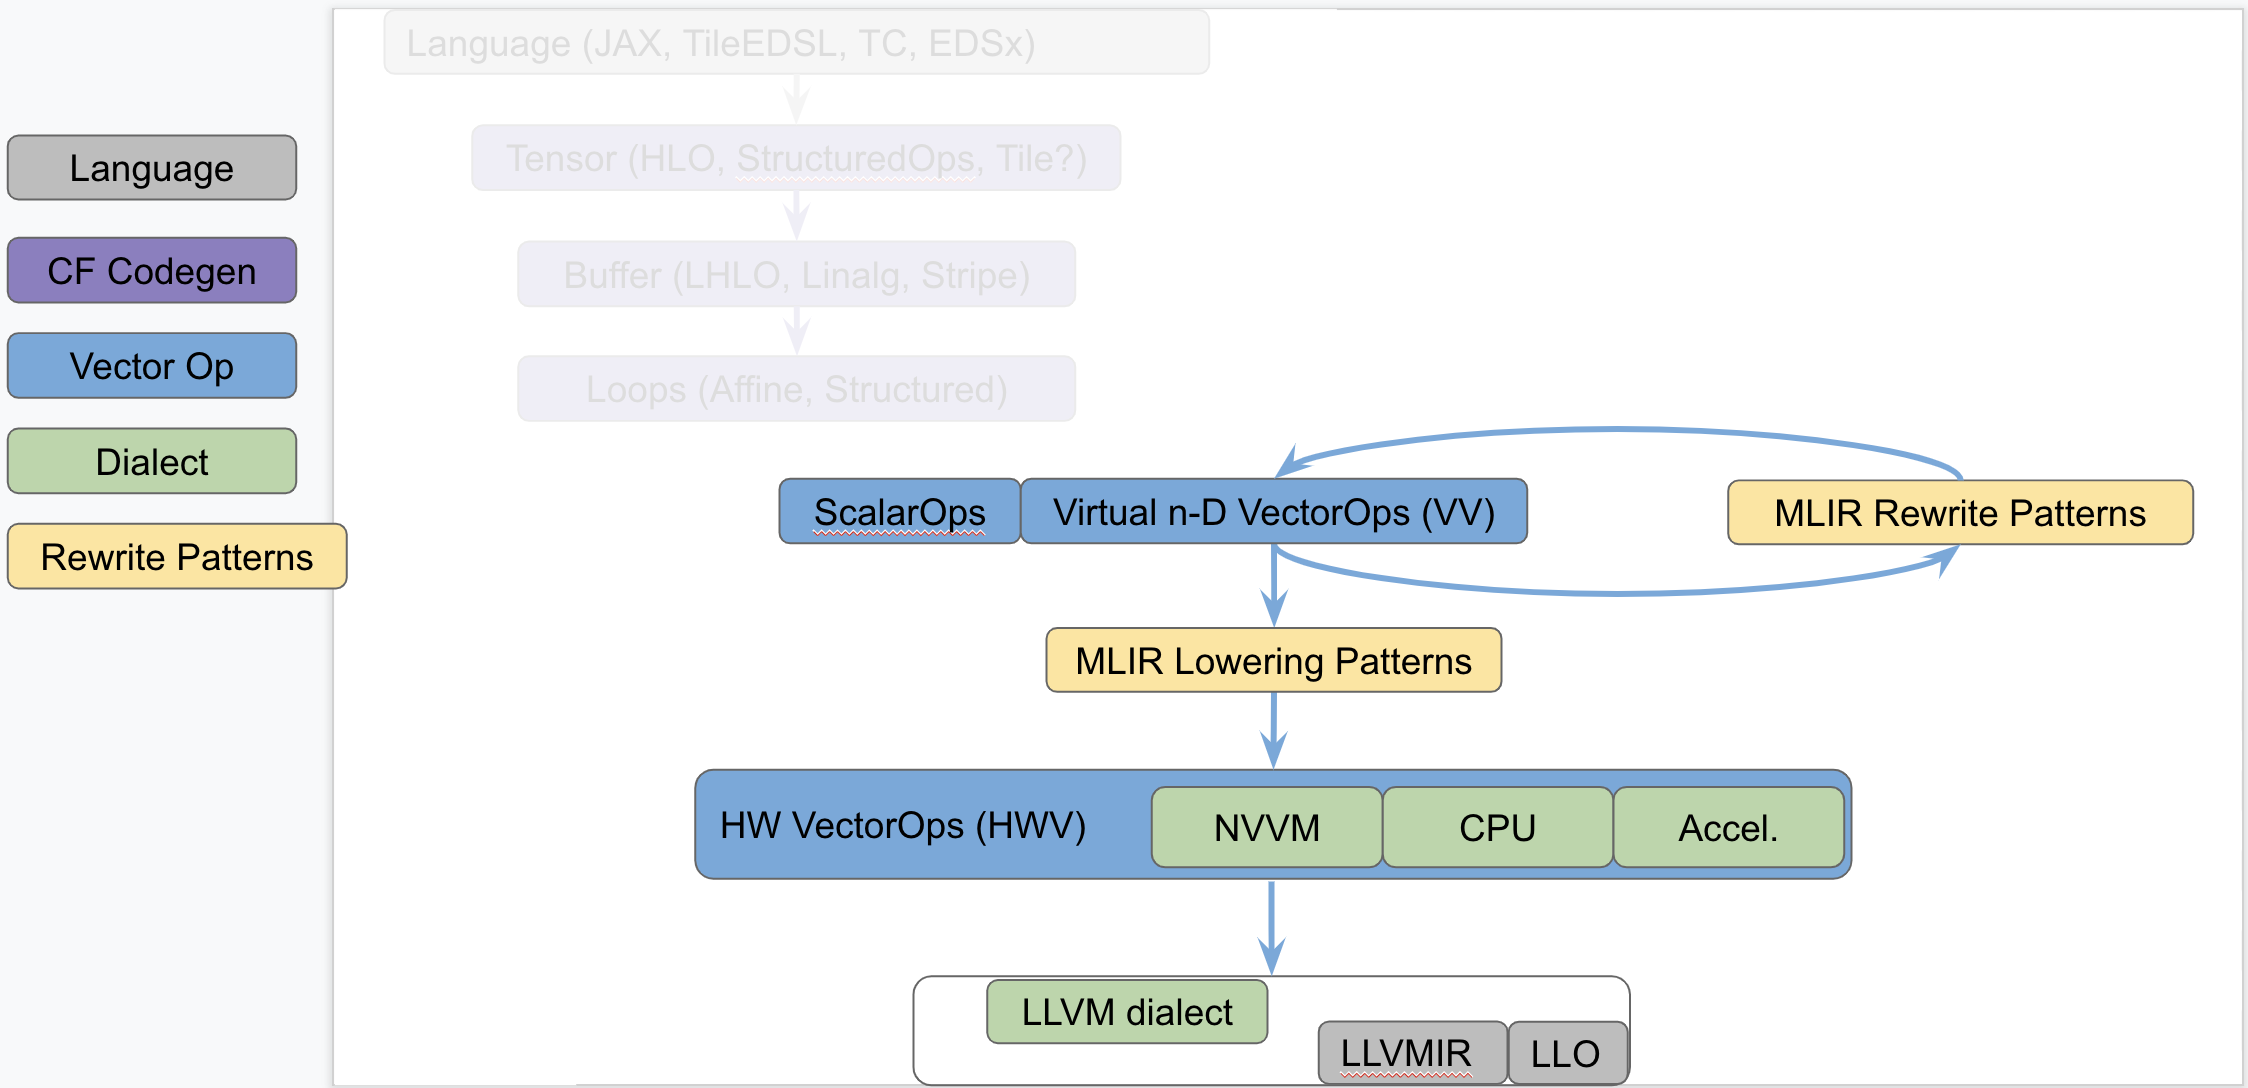
\includegraphics[width=1.0\linewidth]{images/position2.png}
            \caption{MLIR Patterns}
        \end{figure}
    \end{minipage}%
    \hfill%
    \begin{minipage}[t]{0.45\linewidth}
        主要的三层中间表达:
        \begin{enumerate}
            \item Virtual Vector:使用nD vector type,\texttt{vector<4x8x128xf32>}
            \item Hardware Vector:Op $\approx$ 指令
            \item LLVM:instructions,intrinsics, $\dots$
        \end{enumerate}

        \begin{itemize}
            \item VV同层转换:例如unroll,permute
            \item VV $\rightarrow$ HWV,一些手写的pattern:例如CPU的VL;这层lower之后,一些循环优化被禁止(需要确认)
            \item HWV $\rightarrow$ LLVM,手工的
        \end{itemize}
    \end{minipage}



\end{frame}

\begin{frame}
    \frametitle{Auto-Vectorization $\Rightarrow$ Pattern-Rewrite?}

    总体思路:自动向量化 $\rightarrow$ 将标量提升为 Vector 类型 $\rightarrow$ Aseembly

    \hspace{2em}

    如果源代码:
    \begin{enumerate}
        \item 矩阵乘法等高维形式: DSL $\rightarrow$ \texttt{linalg} $\rightarrow$ \texttt{vector}
        \item 标量循环: \texttt{affine.for} $\rightarrow$ \texttt{vector}
    \end{enumerate}

    \begin{center}
        挑战:如何将标量循环转换为 \texttt{vector} ?

        \vspace{1.5em}

        \texttt{SuperVectorize.cpp}
    \end{center}

\end{frame}

\end{document}

